% Provenance (never printed): see sources/outline_sources.md (Year 3: gravitational
% potential, spherical harmonics, J2, reference ellipsoid, geoid, satellite gravimetry,
% flexure of the lithosphere). Brief: sources/book5/BRIEFS.md, ch. 3. Curves from
% figdata/bachelor-3/hydrostatic_figure.py, ice_mass.py (IMBIE 2021), flexure.py.
% Exercise and problem values in the Book 5 scratch calculator calc/ch03.py.
\chapter{الجاذبية وشكل الأرض}\label{ch:b3:gravity-geodesy}

يدور قمران صناعيان أحدهما خلف الآخر حول الأرض، على ارتفاع يزيد على
\qty{500}{km} ويفصل بينهما نحو \qty{220}{km}، ويقيسان المسافة بينهما
باستمرار بدقّة تصل إلى ميكرومتر واحد.
% ledger: geod5:grace, geod5:grace-ranging
عندما يمرّان فوق مكان تتركّز فيه الكتلة، يُسحب القمر المتقدّم إلى الأمام أوّلًا فيتّسع
الفاصل بينهما؛ ثم يُسحب القمر المتأخّر بدوره
فيضيق الفاصل. ومن هذه التغيّرات الصغيرة، شهرًا بعد شهر منذ عام 2002،
رُسم حقل جاذبية الأرض وهو يتغيّر: فالمياه المخزّنة في
الأحواض النهرية ترتفع وتنخفض مع الفصول، وتفقد الأغطية الجليدية الكبرى في
غرينلاند والقارة القطبية الجنوبية كتلتها عامًا بعد عام. وتَزِن الجاذبية ما تعجز العين
عن رؤيته. يبني هذا الفصل حقل الجاذبية لكوكب دوّار انطلاقًا من جهده،
يستخرج منه التفلطح وعزم القصور الذاتي، ويتتبّع
شذوذاته حتى المدار، ثم ينتقل إلى أحد ما تكشفه الجاذبية عند
السطح: \omterm{def:b3:gravity-geodesy:flexure}{انثناء الغلاف الصخري} تحت ثقل بركان.

\begin{recall}
قانون نيوتن للتجاذب الكوني، وطاقة الكمون الجذبي،
والقوة الطاردة المركزية في إطار دوّار هي من كتب الفيزياء؛ وعزوم القصور الذاتي
لجسم صلب وكثيرات حدود ليجندر $P_2(x) = (3x^2 - 1)/2$ واردة في
المجلّدات الجامعية لكتب الفيزياء والرياضيات، ومعامل يونغ $E$
ونسبة بواسون $\nu$ في مجلّد السنة الثالثة لكتب الفيزياء. وقد عُرفت الجيوديسيا
والتفلطح $f = (a - b)/a$ للإهليلجي ذي نصفي المحورين $a > b$ في
الصف العاشر. وعُرّف التوازن الأيزوستاتي، والتعويض الأيري، والجاذبية المرجعية، والجيود،
وارتفاع الجيود، وشذوذات الجاذبية في مجلّد السنة الأولى، في فصله
المخصّص للتوازن الأيزوستاتي وشذوذات الجاذبية.
\end{recall}

\section{الجهد الأرضي}

على كوكب دوّار يشعر الجسم الساكن بجذب كتلة الكوكب
وبالقوة الطاردة المركزية في الإطار الدوّار معه. وكلاهما يشتقّ من
جهدٍ واحد.

\begin{definition}[الجهد الأرضي]\label{def:b3:gravity-geodesy:geopotential}
\emph{الجهد الأرضي}\index{الجهد الأرضي} هو طاقة الكمون لكلّ وحدة
كتلة، في الإطار الدوّار مع الأرض بالسرعة الزاوية $\omega$، للجذب
والقوة الطاردة المركزية معًا:
\[
  W(\mathbf r) = V(\mathbf r) + \Phi(\mathbf r),\qquad
  V(\mathbf r) = -G\int_{\text{الأرض}}\frac{\mathrm dm'}{|\mathbf r - \mathbf r'|},\qquad
  \Phi(\mathbf r) = -\tfrac12\omega^2 s^2,
\]
حيث $s$ هو البعد عن محور الدوران. والجاذبية
$\mathbf g = -\nabla W$، والسطوح $W = \text{ثابت}$ هي سطوحه المتساوية الجهد:
الجاذبية عمودية عليها في كلّ مكان.
\end{definition}

يتدلّى الخيط الشاقولي على امتداد $-\nabla W$، ويستقرّ الماء الساكن على سطح
متساوي الجهد. ومنه يأخذ كوكب مائع دوّار شكل أحد سطوحه
المتساوية الجهد: فالكمون الطارد المركزي، الأعمق عند خطّ الاستواء، يُضخّم
خطّ الاستواء ويُفلطح القطبين.

\begin{omfigure}
\begin{tikzpicture}[font=\small, x=1cm, y=1cm]
\draw[gray, densely dashed] (0,0) circle (2.4);
\draw[very thick, blue!60!black] (0,0) ellipse (2.75 and 2.1);
\draw[->, thick] (0,-2.7) -- (0,2.9) node[above] {محور الدوران};
\draw[gray] (-3.2,0) -- (3.2,0);
\fill (0,0) circle (1.6pt);
% a point at latitude 40 deg (parameter) on the ellipse; the attraction points at
% the centre, the centrifugal force is horizontal, and their sum is drawn along the
% inward normal of the ellipse: lengths solved so that the sum is normal (calc/ch03_fig.py)
\coordinate (P) at (2.107,1.350);
\fill (P) circle (1.8pt);
\draw[->, thick, red!70!black] (P) -- (1.012,0.650);
\node[font=\scriptsize, red!70!black, anchor=south east] at (1.50,1.02) {الجذب};
\draw[->, thick, orange!80!black] (P) -- (2.565,1.350) node[right, font=\scriptsize] {الطاردة المركزية};
\draw[gray, densely dotted] (1.012,0.650) -- (1.470,0.650);
\draw[->, very thick, green!45!black] (P) -- (1.470,0.650);
\node[font=\scriptsize, green!45!black, anchor=north] at (1.470,0.600) {الجاذبية};
\node[blue!60!black, anchor=west, font=\scriptsize] at (2.4,-1.7) {سطح متساوي الجهد};
\node[gray!40!black, anchor=east, font=\scriptsize] at (-1.9,-2.2) {الكرة};
\end{tikzpicture}

\par\smallskip{\small سطح متساوي الجهد لكوكب دوّار (تخطيطيًّا، مع تضخيم
التفلطح تضخيمًا كبيرًا). عند كلّ نقطة، تكون الجاذبية، أي مجموع
الجذب والقوة الطاردة المركزية، عمودية على سطح متساوي الجهد؛ فهي لا
تتّجه نحو المركز إلّا عند القطبين وعلى خطّ الاستواء.}
\label{fig:b3:gravity-geodesy:equipotential}
\end{omfigure}

خارج الكوكب يحقّق الجهد الجذبي معادلة لابلاس،
وحلوله المنتظمة عند اللانهاية هي التوافقيات الكروية الصلبة.

\begin{proposition}[نشر الجهد الأرضي بالتوافقيات الكروية]\label{prop:b3:gravity-geodesy:harmonics}
خارج جسم كتلته $M$ ونصف قطره الاستوائي $a$، ومبدؤه عند مركز كتلته،
ومحوره $z$ على امتداد محور دورانه، يكون الجهد الجذبي
عند المسافة $r$ والزاوية القطبية $\theta$ وخط الطول $\lambda$ هو
\begin{multline*}
  V = -\frac{GM}{r}\Biggl[1 - \sum_{n=2}^{\infty}\left(\frac ar\right)^nJ_nP_n(\cos\theta)\\
  + \sum_{n=2}^{\infty}\sum_{m=1}^{n}\left(\frac ar\right)^nP_{nm}(\cos\theta)
  (C_{nm}\cos m\lambda + S_{nm}\sin m\lambda)\Biggr],
\end{multline*}
مع كثيرات حدود ليجندر $P_n$ والدوال المرافقة $P_{nm}$، والمعاملات
$J_n$، $C_{nm}$، $S_{nm}$ أعداد تُعيَّن بالمطابقة مع الرصد. وبالنسبة إلى
جسم متناظر حول محوره، لا يبقى إلّا الحدود المنطقية $J_n$. ولا يظهر حدّ
من الدرجة 1.
\end{proposition}

\begin{proof}
يُعطي فصل المتغيّرات في معادلة لابلاس في الإحداثيات الكروية
الحلول المنتظمة عند اللانهاية $r^{-(n+1)}$ مضروبًا في $P_{nm}(\cos\theta)e^{\pm
im\lambda}$ (المجلّدات الجامعية لكتب الرياضيات)؛ وأيّ جهد خارج
الكتل هو مجموع هذه الحلول. والحدّ من الدرجة 0 هو $-GM/r$، أي جهد
الكتلة كلّها. والحدود من الدرجة 1 تتناسب مع العزوم الأولى
$\int\mathbf r'\,\mathrm dm'$، وتنعدم هذه عندما يكون المبدأ عند مركز
الكتلة. ويُزيل التناظر المحوري كلّ حدّ يعتمد على $\lambda$.
\end{proof}

\begin{definition}[معامل الشكل الديناميكي]\label{def:b3:gravity-geodesy:j2}
\emph{معامل الشكل الديناميكي}\index{معامل الشكل الديناميكي} $J_2$ لكوكبٍ ما
هو معامل الحدّ الزونالي التوافقي من الدرجة 2، أي أكبر انحراف لجهده الخارجي
عن جهد الكرة، وذلك بسبب تفلطحه. وبالنسبة إلى
الأرض، $J_2 = \num{1.08263e-3}$.
% ledger: geod5:grs80-defining
\end{definition}

\begin{theorem}[صيغة ماكولا]\label{thm:b3:gravity-geodesy:maccullagh}
لتكن $A$، $B$، $C$ عزوم القصور الذاتي الرئيسية لجسمٍ كتلته $M$
حول محاور تمرّ بمركز كتلته، و$I$ عزم قصوره الذاتي حول
المستقيم الواصل من مركز الكتلة إلى نقطة خارجية على بعد $r$. وحتى الرتبة
$r^{-3}$ يُعطى الجهد الثقالي عند تلك النقطة وفق
\emph{صيغة ماكولا}\index{صيغة ماكولا}
\[
  V = -\frac{GM}{r} - \frac{G(A + B + C - 3I)}{2r^3} .
\]
وبالنسبة إلى جسم متماثل حول المحور $z$ ($A = B$)،
$V = -\dfrac{GM}{r} + \dfrac{G(C - A)}{r^3}P_2(\cos\theta)$، ومنه
\[
  J_2 = \frac{C - A}{Ma^2} .
\]
\end{theorem}

\begin{proof}
وليكن $\hat{\mathbf r}$ متجهة الوحدة الموجَّهة نحو النقطة، و$r' \ll r$،
\[
  \frac{1}{|\mathbf r - \mathbf r'|} = \frac1r + \frac{\hat{\mathbf r}\cdot\mathbf r'}{r^2}
  + \frac{3(\hat{\mathbf r}\cdot\mathbf r')^2 - r'^2}{2r^3} + O(r^{-4}).
\]
بالتكامل على الكتلة، يُعطي الحدّ الأوّل $M/r$، وينعدم الحدّ الثاني
(مركز الكتلة). وفي الحدّ الثالث، $\int r'^2\,\mathrm dm' = (A + B + C)/2$، لأنّ
$A + B + C = \int 2r'^2\,\mathrm dm'$، و$\int(\hat{\mathbf r}\cdot\mathbf
r')^2\,\mathrm dm' = \int r'^2\,\mathrm dm' - I$، ومربّع المسافة إلى
المستقيم هو $r'^2 - (\hat{\mathbf r}\cdot\mathbf r')^2$. ويساوي تكامل القوس
$3(A + B + C)/2 - 3I - (A + B + C)/2 = A + B + C - 3I$. وعند $A = B$، يكون العزم
حول مستقيم عند الزاوية المتمّمة لخط العرض $\theta$ هو $I = A\sin^2\theta + C\cos^2\theta$،
و$2A + C - 3I = (C - A)(1 - 3\cos^2\theta) = -2(C - A)P_2(\cos\theta)$.
وبمقارنة ذلك مع \cref{prop:b3:gravity-geodesy:harmonics} نجد
$J_2Ma^2 = C - A$.
\end{proof}

ومن ثمّ يقيس الحدّ من الدرجة 2 في الجهد الفرقَ بين
عزمَي القصور الذاتي، لا العزوم نفسها. أمّا تقدّم محور الأرض،
الذي تدفعه عزوم الشمس والقمر المؤثّرة في الانتفاخ الاستوائي،
يقيس الإهليلجية الديناميكية $H = (C - A)/C$؛ وبالجمع بين $J_2$ و$H$ نحصل على
$C/(Ma^2)$، وهو عامل عزم القصور الذاتي، ويساوي \num{0.3308} للأرض،
% ledger: earth:MoI
أدنى بكثير من \num{0.4} الخاصّة بالكرة المتجانسة: إذ تتركّز الكتلة نحو
المركز.

\section{الإهليلجي الدوّار}

\begin{definition}[الإهليلجي المرجعي]\label{def:b3:gravity-geodesy:ellipsoid}
\emph{الإهليلجي المرجعي}\index{الإهليلجي المرجعي} هو إهليلجي دوراني،
ذا نصف المحور الاستوائي $a$ والتفلطح $f$، ويُختار بحيث يكون
هو نفسه سطح تساوي جهدٍ نموذجيّ: جهدُ جسمٍ دوّار
كتلته $M$ بالسرعة الزاوية $\omega$ \omterm{def:b3:gravity-geodesy:j2}{ومعامل الشكل الديناميكي}
$J_2$ للأرض. وتحدّد هذا الإهليلجي أربعةُ ثوابت؛ ويأخذ نظام المرجع الجيوديسي
1980 القيم الآتية:
\begin{gather*}
  a = \qty{6378137}{m},\qquad GM = \qty{3.986005e14}{m^3.s^{-2}},\\
  J_2 = \num{1.08263e-3},\qquad \omega = \qty{7.292115e-5}{rad.s^{-1}},
\end{gather*}
ومنها يُشتقّ التفلطح $f = \num{0.00335281068}$
($1/f = \num{298.257222}$) ونصف المحور الصغير
$b = \qty{6356752.3141}{m}$.
% ledger: geod5:grs80-defining, geod5:grs80-derived
\end{definition}

يُعرف جهدُ النموذج، أي الجهد المرجعي، على صورة مغلقة، وكذلك
جاذبيتُه على الإهليلجي، أي الجاذبية المرجعية في مجلد السنة الأولى.

\begin{proposition}[صيغة سوميليانا]\label{prop:b3:gravity-geodesy:somigliana}
على إهليلجي مرجعي ذي نصفي المحورين $a$ و$b$، والجاذبية المرجعية
$\gamma_e$ عند خط الاستواء و$\gamma_p$ عند القطبين تُعطى عند
خط العرض الجيوديسي $\varphi$ بالعلاقة
\emph{صيغة سوميليانا}\index{صيغة سوميليانا}
\[
  \gamma(\varphi) = \frac{a\gamma_e\cos^2\varphi + b\gamma_p\sin^2\varphi}
  {\sqrt{a^2\cos^2\varphi + b^2\sin^2\varphi}} .
\]
بالنسبة إلى نظام المرجع الجيوديسي 1980، $\gamma_e = \qty{9.7803267715}{m.s^{-2}}$
و$\gamma_p = \qty{9.8321863685}{m.s^{-2}}$، والسلسلة
$\gamma = 9.780327(1 + 0.0053024\sin^2\varphi - 0.0000058\sin^22\varphi)$
\unit{m.s^{-2}} تُطابق الصيغة إلى حدود \qty{0.1}{\milli\gal}.
% ledger: geod5:grs80-derived, moritz:grs80 (Book 3, read-only)
\end{proposition}
\admitted

ما مقدار التفلطح الذي ينبغي أن يبلغه كوكبٌ دوّار؟ إذا كان مائعًا في
التوازن الهيدروستاتيكي، فإنّ تفلطحه يتحدّد بدورانه وبكيفية توزّع كتلته
في العمق.

\begin{proposition}[علاقتا كلّيرو ودارون--رادو]\label{prop:b3:gravity-geodesy:clairaut}
لكوكب في توازن هيدروستاتيكي، ولتكن $m = \omega^2a^2b/(GM)$ هي نسبة
التسارع النابذ إلى التسارع الثقالي عند خط الاستواء، وحتى الرتبة الأولى في
$f$ و$m$:
\[
  J_2 = \frac{2f - m}{3}\qquad\text{(كلّيرو)},\qquad
  \frac{C}{Ma^2} = \frac23\left[1 - \frac25\sqrt{\frac52\frac mf - 1}\right]
  \qquad\text{(دارون--رادو)} .
\]
الكوكب المتجانس ($C/Ma^2 = 0.4$) يتحقّق فيه $f = 5m/4$؛ أمّا كوكب تتركّز كتلته
نحو المركز فيكون أقلّ تفلطحًا.
\end{proposition}
\admitted

تُحوّل علاقةُ كلّيرو، مع $m = \num{0.00344979}$ الخاصّ بالأرض، قيمةَ
$J_2$ المقاسة إلى $f = \num{0.0033488}$، أو $1/298.6$: ضمن
\qty{0.12}{\percent} من تفلطح الإهليلجي. وأمّا علاقة دارون--رادو
مع عامل عزم القصور الذاتي، تُعطي التفلطحَ الذي كانت ستبلغه الأرض
لو كانت مائعًا في توازن: $1/299.9$، مقابل
$1/298.26$ المقاسة. والأرض أكثر تفلطحًا قليلًا من كوكب مائع بدورانه
وتوزيع كتلته؛ فانتفاخها الاستوائي يعلو بنحو
\qty{116}{m} فوق ما يتنبّأ به التوازن الهيدروستاتيكي. والأرض ليست
تمامًا مائعًا في توازن، والفرقُ الصغير بحدّ ذاته
قياسٌ للإجهادات التي يتحمّلها باطنها.

\begin{omfigure}
\begin{tikzpicture}
\begin{axis}[omrecord, width=0.74\linewidth, height=0.44\linewidth,
  xmin=0.3, xmax=0.4, ymin=225, ymax=340,
  xlabel={عامل عزم القصور الذاتي $C/(Ma^2)$}, ylabel={الهيدروستاتيكي $1/f$},
  xtick={0.30,0.32,0.34,0.36,0.38,0.40},
  xticklabel style={/pgf/number format/fixed, /pgf/number format/precision=2}]
\addplot[blue!70!black, thick] table[x=moi, y=f_inv] {figdata/out/bachelor-3-hydrostatic_figure-curve.dat};
\draw[gray, densely dashed] (axis cs:0.3308,225) -- (axis cs:0.3308,299.88);
\draw[gray, densely dashed] (axis cs:0.3,299.88) -- (axis cs:0.3308,299.88);
\fill[blue!70!black] (axis cs:0.3308,299.88) circle (2pt);
\node[font=\scriptsize, anchor=south west] at (axis cs:0.3315,301) {\foreignlanguage{arabic}{الأرض الهيدروستاتيكية، $1/f = 299.9$}};
\draw[red!70!black, thick] (axis cs:0.3,298.26) -- (axis cs:0.4,298.26);
\node[font=\scriptsize, anchor=north east, red!70!black] at (axis cs:0.399,296.5) {\foreignlanguage{arabic}{الأرض المقاسة، $1/f = 298.26$}};
\fill (axis cs:0.4,231.9) circle (2pt);
\node[font=\scriptsize, anchor=east] at (axis cs:0.397,233) {كوكب متجانس};
\end{axis}
\end{tikzpicture}

\par\smallskip{\small تفلطح كوكب مائع بدوران الأرض،
مقابل عامل عزم القصور الذاتي له، من علاقة دارون--رادو
(محسوب من \babelsublr{Geodetic Reference System 1980}). وكلّما ازداد تركّز الكتلة
نحو المركز صار الكوكب أكثر استدارة. وعند قيمة الأرض
\num{0.3308} يكون التفلطح الهيدروستاتيكي $1/299.9$، أقلّ قليلًا من
$1/298.26$ المقاسة.}
\label{fig:b3:gravity-geodesy:hydrostatic}
\end{omfigure}

\section{الجيود والجهد المُضطرِب}

الجيود هو السطح المتساوي الجهد للجهد الأرضي الحقيقي الذي ينطبق
على متوسط مستوى سطح البحر؛ أمّا \omterm{def:b3:gravity-geodesy:ellipsoid}{الإهليلجي المرجعي} فهو سطح متساوي
الجهد الطبيعي $U$ ذي القيمة نفسها، $U_0 = W_0$. أمّا فصلهما،
أي ارتفاع الجيود $N$، فيتحدّد بفرق الجهدين.

\begin{proposition}[صيغة برونس]\label{prop:b3:gravity-geodesy:bruns}
ليكن $T = W - U$ الجهد المُضطرِب. يُعطى ارتفاع الجيود عند نقطة
وفق \emph{صيغة برونس}\index{صيغة برونس}:
\[
  N = -\frac{T}{\gamma},
\]
حيث يُحسب $T$ على الجيود، و$\gamma$ هي الجاذبية المرجعية هناك. أمّا
فائض الكتلة الذي يُعمّق الجهد ($T < 0$)، فيرفع الجيود.
\end{proposition}

\begin{proof}
ليكن P على الجيود وQ النقطةَ الواقعةَ على الإهليلجي تحتها، على بُعد
$N$. لأنّ $U$ يتزايد نحو الخارج بالمعدّل $\gamma$،
$U(\mathrm P) = U(\mathrm Q) + \gamma N = U_0 + \gamma N$. ثمّ
$W_0 = W(\mathrm P) = U(\mathrm P) + T(\mathrm P) = U_0 + \gamma N + T$،
و$W_0 = U_0$ يُعطي $N = -T/\gamma$.
\end{proof}

يقابل ارتفاعَ الجيود \qty{50}{m} فرقُ جهدٍ قدرُه فقط
\qty{490}{J.kg^{-1}}، أي جزءًا واحدًا من \num{e5} من \omterm{def:b3:gravity-geodesy:geopotential}{الجهد الأرضي}. وتتراوح ارتفاعات الجيود
للأرض من نحو $+\qty{85}{m}$ في آيسلندا إلى
$-\qty{106}{m}$ في جنوب الهند،
% ledger: nasa:geoid-range (Book 3, read-only)
أي مدًى دون \qty{200}{m} على كوكب يختلف نصفا قطريه الاستوائي والقطبي
بمقدار \qty{21}{km}.

\section{قياس الجاذبية بالأقمار الصناعية}

\begin{definition}[قياس الجاذبية بالأقمار الصناعية]\label{def:b3:gravity-geodesy:satgrav}
\emph{قياس الجاذبية بالأقمار الصناعية}\index{قياس الجاذبية بالأقمار الصناعية} يحدّد حقل الجاذبية الأرضي
من حركة الأقمار الصناعية: من الاضطرابات طويلة الأمد
لمداراتها، ومن تغيّر المسافة بين قمرين صناعيين على المدار نفسه،
أو من مقاييس التدرّج التي تقيس فروق الجاذبية عبر
المركبة الفضائية.
\end{definition}

أكبر اضطراب لمدار قريب من الأرض يأتي من $J_2$. ويمارس
الانتفاخ الاستوائي عزمًا على المدار المائل، فيدور ببطء
حول محور الأرض.

\begin{proposition}[التقدّم العقدي]\label{prop:b3:gravity-geodesy:nodal}
إلى الرتبة الأولى في $J_2$، يدور خطّ العقد لمدار دائري نصف قطره $r$
وميله $i$ بالمعدّل
\[
  \dot\Omega = -\frac32\,nJ_2\left(\frac ar\right)^2\cos i,\qquad n = \sqrt{GM/r^3} ,
\]
يتجه غربًا في المدار المباشر ($i < \ang{90}$)، ويتجه شرقًا في المدار الرجعي.
\end{proposition}

\begin{proof}
عبر دورات كثيرة يتصرّف القمر الصناعي كحلقة كتلتها $m_s$ موزّعة على
مداره. يُكتب الجزء ذو الدرجة 2 من الجهد،
$(GMJ_2a^2/r^3)P_2(\cos\theta)$ لكلّ وحدة كتلة، متوسّطًا على دائرة مائلة
بميل $i$، يتضمّن $\langle\cos^2\theta\rangle = \tfrac12\sin^2i$، فإنّ
$\langle P_2\rangle = \tfrac34\sin^2i - \tfrac12$، وطاقة الحلقة هي
$E(i) = m_s(GMJ_2a^2/r^3)(\tfrac34\sin^2i - \tfrac12)$. ويكون العزم حول خطّ
العقد هو $\tau = -\mathrm dE/\mathrm di = -\tfrac32m_s(GMJ_2a^2/r^3)\sin
i\cos i$. وهو عمودي على كمية الحركة الزاوية للحلقة $L = m_snr^2$، لذلك
يدير $\mathbf L$ حول المحور القطبي دون أن يغيّر طولها:
$L\sin i\,\dot\Omega = \tau$. ومع $GM = n^2r^3$، فإنّ $\dot\Omega =
-\tfrac32nJ_2(a/r)^2\cos i$.
\end{proof}

يبلغ المعدّل عدّة درجات في اليوم لمدار منخفض قرب خطّ الاستواء؛ وعند ميل
قليلًا بعد \ang{90} يتطابق مع الحركة السنوية للشمس، ويحتفظ
المدار بالتوجّه نفسه نحو الشمس طوال السنة (انظر التمرين 12). وعند القياس على
أقمار صناعية كثيرة بميول مختلفة، تُعطي هذه التقدّمات $J_2$
والتوافقيات المنطقية الأعلى.

يؤدّي زوج من الأقمار الصناعية أفضل: إذ يقيس تغيّر المسافة بينهما
فرق الجاذبية التي يشعران بها على طول المدار. طار زوج GRACE من 2002 إلى 2017،
وخلَفه \babelsublr{GRACE Follow-On}، منذ إطلاقه في 22 مايو 2018، وتقيس وصلته الميكروويفية
المسافة بدقّة في حدود الميكرومتر، ووصلة ليزرية تختبر
دقّةً تصل إلى عشرين مرّة أفضل.
% ledger: geod5:grace, geod5:grace-ranging
يتغيّر الحقل من شهر إلى آخر لأنّ الماء يتحرّك: الثلج ورطوبة
التربة، والمياه الجوفية، والبحيرات، والمحيطات، والغطاء الجليدي.

\begin{omfigure}
\begin{tikzpicture}[font=\small, x=1cm, y=1cm]
\draw[thick, brown!60!black] (-5,0) -- (1.6,0) .. controls (2.0,0.08) and (3.0,0.08) .. (3.4,0) -- (5,0);
\fill[blue!25] (1.8,0) rectangle (3.2,-0.6);
\node[font=\scriptsize] at (2.5,-0.3) {كتلة زائدة};
\draw[gray, densely dashed] (-5,2.5) -- (5,2.5);
\node[gray!40!black, font=\scriptsize, anchor=south west] at (-5,2.55) {المدار};
\fill[orange!80!black] (-2.6,2.35) rectangle (-2.0,2.65);
\fill[orange!80!black] (0.4,2.35) rectangle (1.0,2.65);
\draw[<->, red!70!black, thick] (-1.95,2.5) -- (0.35,2.5) node[midway, above, font=\scriptsize] {\foreignlanguage{arabic}{المدى، نحو \mbox{\textdir TLT \qty{220}{km}}}};
\draw[->, thick] (0.85,2.3) -- (1.45,1.75);
\draw[->, thick, gray] (2.6,2.9) -- (4.2,2.9) node[right, font=\scriptsize] {الحركة};
\node[font=\scriptsize, anchor=north, align=center] at (0.2,1.6) {\foreignlanguage{arabic}{القمر المتقدّم يُسحب إلى الأمام أولًا:}\\يتّسع المدى};
\node[font=\scriptsize, anchor=north, align=center] at (-2.9,1.6) {\foreignlanguage{arabic}{لاحقًا يُسحب القمر المتأخّر إلى الأمام أيضًا:}\\يضيق المدى};
\end{tikzpicture}

\par\smallskip{\small مبدأ زوج الأقمار الصناعية (تخطيطي، ليس
بمقياس الرسم). عند الاقتراب من كتلة زائدة، يشعر القمر المتقدّم بجذبها
أولًا ويُعجَّل نحو الأمام، فيزداد المدى بينهما؛ وعندما
يمرّ القمر المتأخّر فوق الكتلة فيتناقص المدى من جديد. ومعدّل
تغيّر المدى المقاس باستمرار يُعكس لاستنتاج حقل الجاذبية.}
\label{fig:b3:gravity-geodesy:grace}
\end{omfigure}

\begin{omfigure}
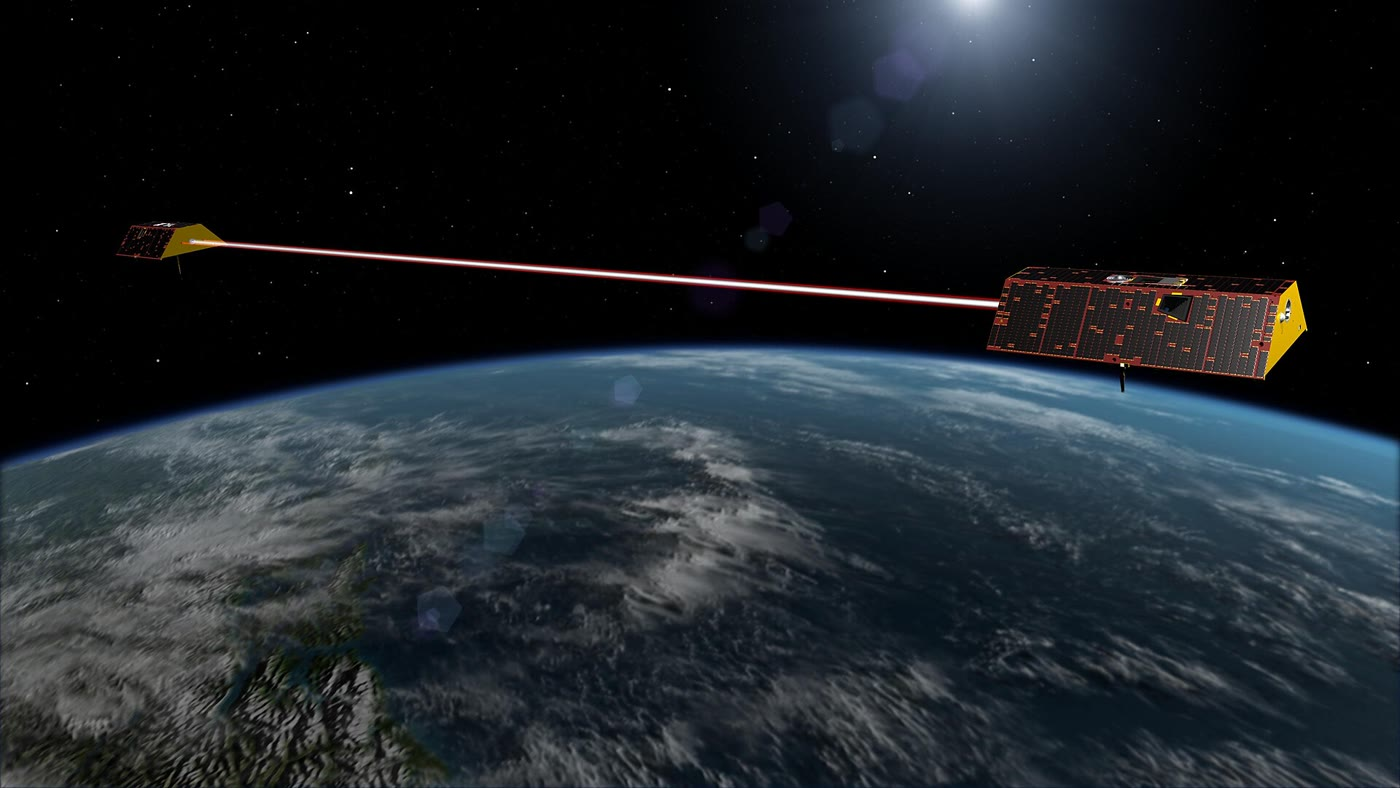
\includegraphics[width=0.66\linewidth]{images/book5/b3-grace-fo-concept.jpg}

\par\smallskip{\small القمران الصناعيان \babelsublr{GRACE Follow-On}، تصوّر فنّي (المسافة
بينهما مختصرة كثيرًا). يرمز الشعاع الأحمر إلى وصلة
القياس بالليزر. \mbox{\textdir TLT NASA/JPL-Caltech}، ملك عام.}
\label{fig:b3:gravity-geodesy:grace-photo}
\end{omfigure}

\begin{definition}[ارتفاع الماء المكافئ]\label{def:b3:gravity-geodesy:ewh}
يمكن تمثيل تغيّر حقل الجاذبية الذي يتغيّر ببطء على مسافات أكبر بكثير
من سمك الطبقة التي تحرّكت فيها الكتلة بتغيّر في الكثافة السطحية
$\sigma$ (\unit{kg.m^{-2}}) على قشرة رقيقة عند
سطح الأرض. يُسمّى \emph{ارتفاع الماء المكافئ}\index{ارتفاع الماء المكافئ}
هو سمك الماء العذب الذي له الكثافة السطحية نفسها:
\[
  h_w = \frac{\sigma}{\rho_w} .
\]
\end{definition}

متر واحد من الماء فوق حوض مساحته \qty{1e6}{km^2} يساوي \qty{1e15}{kg}، أو
\qty{1000}{Gt}. مستوى سطح البحر هو الطرف الآخر من الميزانية: \qty{360}{Gt} من الجليد
يُضاف إلى المحيط يرفعه بنحو ملّيمتر واحد.
% ledger: data:b5-imbie
\omterm{def:b3:gravity-geodesy:satgrav}{قياس الجاذبية بالأقمار الصناعية}، وقياس الارتفاع بالأقمار الصناعية، وحصيلة تساقط الثلج مقابل
تصريف الجليد، تقيس كلٌّ منها الحصيلة الكتلية للغطاء الجليدي؛ وبعد التوفيق بينها،
تُعطي السلسلة الآتية.

\begin{omfigure}
\begin{tikzpicture}
\begin{axis}[omrecord, width=0.82\linewidth, height=0.5\linewidth,
  xmin=1992, xmax=2021, ymin=-5600, ymax=600,
  xlabel={السنة}, ylabel={التغيّر التراكمي للكتلة \babelsublr{(\unit{Gt})}},
  xticklabel style={/pgf/number format/1000 sep={}},
  legend pos=south west, legend cell align=left, legend style={font=\scriptsize}]
\addplot[name path=gl, draw=none, forget plot] table[x=year, y=lo] {figdata/out/bachelor-3-ice_mass-greenland.dat};
\addplot[name path=gh, draw=none, forget plot] table[x=year, y=hi] {figdata/out/bachelor-3-ice_mass-greenland.dat};
\addplot[blue!25, forget plot] fill between[of=gl and gh];
\addplot[name path=al, draw=none, forget plot] table[x=year, y=lo] {figdata/out/bachelor-3-ice_mass-antarctica.dat};
\addplot[name path=ah, draw=none, forget plot] table[x=year, y=hi] {figdata/out/bachelor-3-ice_mass-antarctica.dat};
\addplot[red!20, forget plot] fill between[of=al and ah];
\addplot[blue!70!black, thick] table[x=year, y=cum] {figdata/out/bachelor-3-ice_mass-greenland.dat};
\addlegendentry{غرينلاند}
\addplot[red!70!black, thick] table[x=year, y=cum] {figdata/out/bachelor-3-ice_mass-antarctica.dat};
\addlegendentry{أنتاركتيكا}
\draw[gray, densely dotted] (axis cs:2002.25,-5600) -- (axis cs:2002.25,600);
\draw[gray, densely dotted] (axis cs:2017.5,-5600) -- (axis cs:2017.5,600);
\node[font=\scriptsize, gray!40!black, anchor=north] at (axis cs:2009.9,550) {\foreignlanguage{arabic}{سنوات GRACE}};
\end{axis}
\end{tikzpicture}

\par\smallskip{\small التغيّر التراكمي للكتلة في الغطاءين الجليديين لغرينلاند
وأنتاركتيكا منذ 1992، مع نطاقات بانحراف معياري واحد (تقديرات \babelsublr{IMBIE 2021}
المصالَحة من قياس الارتفاع والجاذبية وطريقة المدخلات--المخرجات). بحلول نهاية
عام 2020 فقدت غرينلاند $\num{4890} \pm \qty{460}{Gt}$ وأنتاركتيكا
$\num{2670} \pm \qty{530}{Gt}$؛ تعطي الملاءمات الخطّية
\qty{-176}{Gt.yr^{-1}} و\qty{-91}{Gt.yr^{-1}} خلال الفترة 1992--2020،
و\qty{-246}{Gt.yr^{-1}} و\qty{-127}{Gt.yr^{-1}} خلال سنوات GRACE.}
\label{fig:b3:gravity-geodesy:ice-mass}
\end{omfigure}

شذوذ الجاذبية المقاس عند السطح هو مجموع توافقيات؛ وعند
ارتفاع قمر صناعي، يضعف كلٌّ منها بعامل يعتمد على
طول موجته.

\begin{proposition}[الاستمرار إلى الأعلى]\label{prop:b3:gravity-geodesy:upward}
فوق الكتل المسبّبة له، يكون شذوذ الجاذبية الذي يتغيّر على طول السطح
بالصيغة $\Delta g_0\cos kx$، حيث $k = 2\pi/\lambda$، عند الارتفاع $z$ (أي
\emph{الاستمرار إلى الأعلى}\index{الاستمرار إلى الأعلى})
\[
  \Delta g(x, z) = \Delta g_0\,e^{-kz}\cos kx .
\]
\end{proposition}

\begin{proof}
فوق الكتل، يحقّق الجهد الشاذّ، ومعه الشذوذ، معادلة
لابلاس $\partial_x^2\Delta g + \partial_z^2\Delta g = 0$. بفصل
المتغيّرات، $\Delta g = Z(z)\cos kx$ مع $Z'' = k^2Z$، وحلّها المحدود عندما
$z \to \infty$ هو $Z = \Delta g_0e^{-kz}$.
\end{proof}

عند ارتفاع \qty{400}{km} يحتفظ شذوذ طوله \qty{1000}{km} بنسبة \qty{8}{\percent}
من سعته، والذي طوله \qty{100}{km} يحتفظ بنحو \num{1e-11} منها:
ترى الأقمار الصناعية الأطوال الموجية الطويلة، وترصد المسوح عند السطح القصيرة.

\section{انثناء الغلاف الصخري}

عوّض مجلد السنة الأولى حملًا محليًا، إذ يطفو كلّ عمود على حدة.
لا يُعوَّض بركانٌ واقعٌ على صفيحة محيطية تحته وحده: تنحني الصفيحة
تحته على عرض مئات الكيلومترات، ويهبط قاع البحر حول البركان في خندقٍ محيطيّ،
وما وراءه يرتفع في قوس منخفض.

\begin{definition}[انثناء الغلاف الصخري، صلابة الانثناء، السمك المرن الفعّال]\label{def:b3:gravity-geodesy:flexure}
\emph{انثناء الغلاف الصخري}\index{انثناء الغلاف الصخري} هو انحناء
الغلاف الصخري تحت حمل، ويُنمذَج بوصفه انحناء صفيحة مرنة رقيقة
طافية على وشاح مائع. ومقاومة الصفيحة للانحناء هي
\emph{صلابة الانثناء}\index{صلابة الانثناء}
\[
  D = \frac{ET_e^3}{12(1 - \nu^2)},
\]
و$T_e$ هو سمك الصفيحة المرنة المتجانسة التي تنحني كما ينحني الغلاف الصخري الحقيقي،
وهو \emph{السمك المرن الفعّال}\index{السمك المرن الفعّال}.
\end{definition}

\begin{theorem}[انثناء صفيحة رقيقة]\label{thm:b3:gravity-geodesy:plate}
صفيحة مرنة رقيقة صلابتها $D$، تنحني في اتجاه واحد بفعل حمل $q(x)$
لكلّ وحدة مساحة، تنحرف نحو الأسفل بمقدار $w(x)$، وتطفو على وشاح كثافته
$\rho_m$، والتجويف مملوء بمادة كثافتها $\rho_i$، فتحقّق
\emph{معادلة الانثناء}\index{معادلة الانثناء}
\[
  D\frac{\mathrm d^4w}{\mathrm dx^4} + (\rho_m - \rho_i)g\,w = q(x) .
\]
\end{theorem}

\begin{proof}
في الصفيحة المنحنية، تتقلّص الألياف الواقعة فوق المستوى المنتصف،
وتتمدّد الواقعة تحته، بما يتناسب مع الانحناء $w''$؛ وبتكامل إجهاد الانحناء
على السمك نحصل على عزم الانحناء $M = -Dw''$، مع
الصلابة الواردة في التعريف (لا تتمدّد الصفيحة جانبيًا، ومن ثمّ المعامل
$1 - \nu^2$؛ انظر مجلد السنة الثالثة من كتب الفيزياء). شريحةٌ $\mathrm dx$ من الصفيحة
تحمل قوة القصّ $V$ على وجهيها والعزم $M$. التوازن الشاقولي:
الحمل $q\,\mathrm dx$ نحو الأسفل، وقوة الطفو للوشاح المُزاح
$(\rho_m - \rho_i)gw\,\mathrm dx$ نحو الأعلى، فيعطي $\mathrm dV/\mathrm dx = -q +
(\rho_m - \rho_i)gw$. وتوازن العزوم يعطي $\mathrm dM/\mathrm dx = V$.
ومنه $-Dw'''' = M'' = V' = -q + (\rho_m - \rho_i)gw$.
\end{proof}

\begin{definition}[معامل الانثناء، الانتفاخ الأمامي]\label{def:b3:gravity-geodesy:alpha}
\emph{معامل الانثناء}\index{معامل الانثناء} لصفيحة ما هو
الطول
\[
  \alpha = \left(\frac{4D}{(\rho_m - \rho_i)g}\right)^{1/4},
\]
الذي يحدّد المقياس الأفقي لانثنائها. \emph{الانتفاخ الأمامي}\index{الانتفاخ الأمامي} هو
القوس المنخفض من الانثناء نحو الأعلى الذي ترفعه الصفيحة المنحنية خارج الخندق المحيطي أو
الحوض المجاور لحملها.
\end{definition}

\begin{proposition}[حمل خطّي على صفيحة متّصلة]\label{prop:b3:gravity-geodesy:line}
يُحدث حمل خطّي $V_0$ لكلّ وحدة طول على امتداد $x = 0$ انحرافًا للصفيحة مقداره
\[
  w(x) = w_0e^{-|x|/\alpha}\left(\cos\frac{|x|}{\alpha} + \sin\frac{|x|}{\alpha}\right),
  \qquad w_0 = \frac{V_0\alpha^3}{8D} .
\]
ينعدم الانحراف عند $|x| = 3\pi\alpha/4$، أي حافّة الخندق المحيطي، وتقع
قمّة \omterm{def:b3:gravity-geodesy:alpha}{الانتفاخ الأمامي} عند $|x| = \pi\alpha$، وارتفاعها $w_0e^{-\pi} =
\num{0.0432}\,w_0$. وتوازن قوةُ الطفو لكامل الانحراف الحملَ:
$\int(\rho_m - \rho_i)gw\,\mathrm dx = V_0$.
\end{proposition}

\begin{proof}
من أجل $x > 0$ تكون المعادلة $w'''' + 4w/\alpha^4 = 0$؛ وجذور
$r^4 = -4/\alpha^4$ هي $(\pm1 \pm i)/\alpha$، والحلول التي تنعدم بعيدًا
هي $e^{-x/\alpha}(A\cos(x/\alpha) + B\sin(x/\alpha))$. وتفرض التناظر
$w'(0) = 0$، وهذا يعطي $A = B = w_0$. وبتكامل التوازن الشاقولي عبر
الحمل، تقفز قوة القصّ $V = -Dw'''$ بمقدار $-V_0$؛ وبالتناظر
$w'''(0^-) = -w'''(0^+)$، و$w'''(0^+) = 4w_0/\alpha^3$، فيكون $8Dw_0/\alpha^3 =
V_0$. وينعدم الانحراف حيث $\tan(x/\alpha) =
-1$، أوّلًا عند $x = 3\pi\alpha/4$؛ ومشتقّته،
$-(2w_0/\alpha)e^{-x/\alpha}\sin(x/\alpha)$، تنعدم بعد ذلك عند $x = \pi\alpha$.
وأخيرًا $\int_0^\infty e^{-u}(\cos u + \sin u)\,\mathrm du = 1$، إذن
$\int w\,\mathrm dx = 2w_0\alpha = V_0\alpha^4/(4D) = V_0/((\rho_m - \rho_i)g)$.
\end{proof}

\begin{proposition}[صفيحة مكسورة]\label{prop:b3:gravity-geodesy:broken}
صفيحةٌ مكسورة عند $x = 0$ ويُدفع طرفها الحرّ نحو الأسفل، كما هو الحال عند خندقٍ
بحريّ عميق، تنحرف وفق $w = w_0e^{-x/\alpha}\cos(x/\alpha)$ من أجل $x \ge 0$:
ينعدم الانحراف عند $x = \pi\alpha/2$، وتقع قمّة \omterm{def:b3:gravity-geodesy:alpha}{الانتفاخ الأمامي}،
أي الارتفاع الخارجي، عند $x = 3\pi\alpha/4$، وارتفاعها $w_0e^{-3\pi/4}/\sqrt2 =
\num{0.067}\,w_0$.
\end{proposition}

\begin{proof}
الحلول المتناقصة نفسها، لكن مع طرف حرّ لا يحمل عزمًا،
$w''(0) = 0$، وهذا يعطي $B = 0$. ويقع الصفر عند $\cos(x/\alpha) = 0$؛
والمشتقّة $-(w_0/\alpha)e^{-x/\alpha}(\cos + \sin)(x/\alpha)$ تنعدم عند
$x = 3\pi\alpha/4$، حيث $w = w_0e^{-3\pi/4}\cos(3\pi/4)$.
\end{proof}

ومن ثمّ فالمسافات هي مفتاح قوّة الصفيحة: يُقاس موضع انتهاء الخندق المحيطي
أو موضع قمّة الانتفاخ، فيُستنتج $\alpha$، ثم $D$، ثم $T_e$.
ولمّا كان $T_e$ يدخل بوصفه $\alpha^{4/3}$، فإنّ تقدير المسافة تقديرًا معقولًا يعطي
تقديرًا جيدًا لسمك الصفيحة.

\begin{omfigure}
\begin{tikzpicture}
\begin{groupplot}[group style={group size=1 by 2, vertical sep=1.5cm},
  width=0.82\linewidth, height=0.36\linewidth, xmin=-400, xmax=400,
  tick label style={font=\scriptsize}, label style={font=\small}, title style={font=\small}]
\nextgroupplot[title={(أ) حمل خطّي: ظهرة أورو على صفائح بثلاث سماكات},
  ylabel={الانحراف \babelsublr{(\unit{m})}}, ymin=-3000, ymax=700, y filter/.expression={-y},
  legend pos=south east, legend cell align=left, legend style={font=\scriptsize}]
\addplot[red!70!black, thick] table[x=x, y=w10] {figdata/out/bachelor-3-flexure-profiles.dat};
\addlegendentry{$T_e = \qty{10}{km}$}
\addplot[blue!70!black, thick] table[x=x, y=w25] {figdata/out/bachelor-3-flexure-profiles.dat};
\addlegendentry{$T_e = \qty{25}{km}$}
\addplot[green!45!black, thick] table[x=x, y=w40] {figdata/out/bachelor-3-flexure-profiles.dat};
\addlegendentry{$T_e = \qty{40}{km}$}
\draw[gray] (axis cs:-400,0) -- (axis cs:400,0);
\draw[->, blue!70!black] (axis cs:222,330) -- (axis cs:222,90);
\node[font=\scriptsize, blue!70!black, anchor=south] at (axis cs:222,330) {\foreignlanguage{arabic}{الانتفاخ الأمامي، $\pi\alpha$}};
\nextgroupplot[title={(ب) صفيحة مكسورة عند خندق، $T_e = \qty{25}{km}$},
  xlabel={المسافة من الحمل أو الخندق \babelsublr{(\unit{km})}},
  ylabel={الانحراف \babelsublr{(\unit{m})}}, xmin=0, xmax=400, ymin=-1100, ymax=280,
  y filter/.expression={-y}]
\addplot[blue!70!black, thick] table[x=x, y=w] {figdata/out/bachelor-3-flexure-broken.dat};
\draw[gray] (axis cs:0,0) -- (axis cs:400,0);
\draw[->] (axis cs:166.5,200) -- (axis cs:166.5,80);
\node[font=\scriptsize, anchor=west] at (axis cs:170,200) {\foreignlanguage{arabic}{الارتفاع الخارجي، $3\pi\alpha/4$}};
\end{groupplot}
\end{tikzpicture}

\par\smallskip{\small انثناء صفيحة مرنة (محسوب؛
$E = \qty{100}{GPa}$، $\nu = 0.25$، الوشاح \qty{3300}{kg.m^{-3}}، الماء في
الحفرة المحيطة؛ مقياس رأسي مبالَغ فيه كثيرًا). (أ) تحت حمل ظهرة بركانية
(\qty{4.17e12}{N.m^{-1}})، تغوص صفيحة رقيقة عميقًا وضيقًا، وتغوص صفيحة
سميكة ضحلًا وعريضًا؛ ينتقل \omterm{def:b3:gravity-geodesy:alpha}{الانتفاخ الأمامي} من \qty{112}{km} إلى
\qty{316}{km}. (ب) صفيحة مكسورة عند خندق ومدفوعة إلى أسفل بمقدار \qty{1}{km}:
يصل الارتفاع الخارجي إلى \qty{67}{m}، على بُعد \qty{167}{km} من الخندق.}
\label{fig:b3:gravity-geodesy:flexure}
\end{omfigure}

\begin{definition}[التعويض الأيزوستاتي الإقليمي]\label{def:b3:gravity-geodesy:regional}
\emph{التعويض الأيزوستاتي الإقليمي}\index{التعويض الأيزوستاتي الإقليمي}
هو إسناد حمل بطفو انحراف ممتدّ على منطقة
أوسع من الحمل، بواسطة \omterm{def:b3:gravity-geodesy:flexure}{صلابة الانثناء} في الغلاف الصخري؛ أمّا في تعويض إيري
أو برات، فيُعوَّض كل عمود تحت ذاته على العكس.
\end{definition}

يوازن التعويضان المحلي والإقليمي الكتلة الكلية نفسها، لكنّهما يوزّعانها
بطريقة مختلفة: تحت حمل ضيق على صفيحة جاسئة يكون الجذر ضحلًا وعريضًا،
ويكون الشذوذ الجاذبي فوق الحمل موجبًا بقوة، يكتنفه من جانبيه شذوذات
سالبة فوق الحفرة المحيطة. وحول جزر ظهرة هاواي تعطي المقاطع الجاذبية
والزلزالية سمكًا مرنًا فعّالًا من 17 إلى \qty{37}{km}،
و10 إلى \qty{20}{km} على طول الجبال البحرية الأقدم في سلسلة الإمبراطور، وهو فرق
يُتوقَّع من أعمار البراكين وأعمار الصفيحة التي حمّلتها؛ وتتبع القيم
عمق خط متساوي الحرارة قرب
\qty{350}{\degreeCelsius} في الصفيحة المحيطية المتبرّدة.
% ledger: watts25:te
يفتح الانثناء نفسه، تحت وزن حزام جبلي، أحواض
المقدّمة في مجلد السنة الثانية، في فصله عن الأوروجين الألبي.

\begin{omfigure}
\begin{tikzpicture}[font=\scriptsize, x=1cm, y=1cm]
\fill[blue!8] (-6,0) rectangle (6,-1.0);
\draw[blue!50!black] (-6,0) -- (6,0) node[right] {مستوى سطح البحر};
% volcano
\fill[brown!45] (-1.2,-1.6) -- (0,0.5) -- (1.2,-1.6) -- cycle;
% moat infill
\fill[yellow!35] (-1.2,-1.6) .. controls (-2.0,-1.5) and (-3.0,-1.15) .. (-3.6,-1.02) -- (-1.2,-1.02) -- cycle;
\fill[yellow!35] (1.2,-1.6) .. controls (2.0,-1.5) and (3.0,-1.15) .. (3.6,-1.02) -- (1.2,-1.02) -- cycle;
% flexed seafloor (top of crust)
\draw[very thick, brown!60!black] (-6,-0.96) .. controls (-5.2,-0.78) and (-4.4,-0.78) .. (-3.6,-1.02)
  .. controls (-3.0,-1.15) and (-2.0,-1.5) .. (-1.2,-1.6) -- (1.2,-1.6)
  .. controls (2.0,-1.5) and (3.0,-1.15) .. (3.6,-1.02) .. controls (4.4,-0.78) and (5.2,-0.78) .. (6,-0.96);
% Moho, parallel
\draw[thick, gray!60!black] (-6,-1.76) .. controls (-5.2,-1.58) and (-4.4,-1.58) .. (-3.6,-1.82)
  .. controls (-3.0,-1.95) and (-2.0,-2.3) .. (-1.2,-2.4) -- (1.2,-2.4)
  .. controls (2.0,-2.3) and (3.0,-1.95) .. (3.6,-1.82) .. controls (4.4,-1.58) and (5.2,-1.58) .. (6,-1.76);
\node[anchor=west] at (4.2,-1.95) {الموهو};
\draw[dashed, gray] (-6,-1.0) -- (6,-1.0);
\node[anchor=north west, gray!40!black] at (-6,-1.03) {قاع المحيط غير المنثني};
\node[anchor=south, align=center] at (-2.6,-0.98) {الحفرة المحيطة\\(الحشو)};
\node[anchor=south] at (4.8,-0.82) {الانتفاخ الأمامي};
\node at (0,-0.6) {البركان};
\node[anchor=north] at (0,-2.5) {\foreignlanguage{arabic}{صفيحة منحنية إلى الأسفل على عرض بضعة $\alpha$}};
\end{tikzpicture}

\par\smallskip{\small جزيرة بركانية على صفيحة محيطية (مقطع عرضي تخطيطي،
مقياس رأسي مبالَغ فيه). تنحني الصفيحة تحت البركان؛
الفجوة المحيطة به، أي الحفرة المحيطة، تمتلئ بالفتات البركاني والرواسب؛
أمّا ما وراءها فترتفع الصفيحة في انتفاخ أمامي منخفض.}
\label{fig:b3:gravity-geodesy:moat}
\end{omfigure}

\begin{inthefield}[مسح جاذبي نسبي]
\begin{minipage}[t]{0.55\linewidth}\vspace{0pt}
يُسقط مقياس الجاذبية المطلق مرآةً مكعبة الزوايا في غرفة مفرغة مرارًا
وتكرارًا، ويقيس زمن سقوطها بمقياس تداخل ليزري وساعة ذرية؛
فيعطي الجاذبية عند محطة واحدة، لكنّه ثقيل وبطيء الإعداد. ويُنجَز المسح
نفسه بمقياس الجاذبية النسبي، وهو ميزان زنبركي صغير يقيس
فروق الجاذبية. يُسوّيه الجيوفيزيائي على لوحة قاعدة عند كل
محطة على امتداد خطّ، فيقرأه ويدوّن الزمن والارتفاع وينتقل إلى التالية؛ وكل
بضع ساعات يعود المسار إلى محطة أساس، فيُقاس الانجراف البطيء للزنبرك
ومدّ الأرض الصلبة ويُزال. ويعطي مستقبِل القمر الصناعي
على عمود قريب الموضعَ والارتفاع، لأنّ الجاذبية
تتغيّر بنحو \qty{0.3}{\milli\gal} مع كل متر من الارتفاع.
\end{minipage}\hfill
\begin{minipage}[t]{0.42\linewidth}\vspace{0pt}
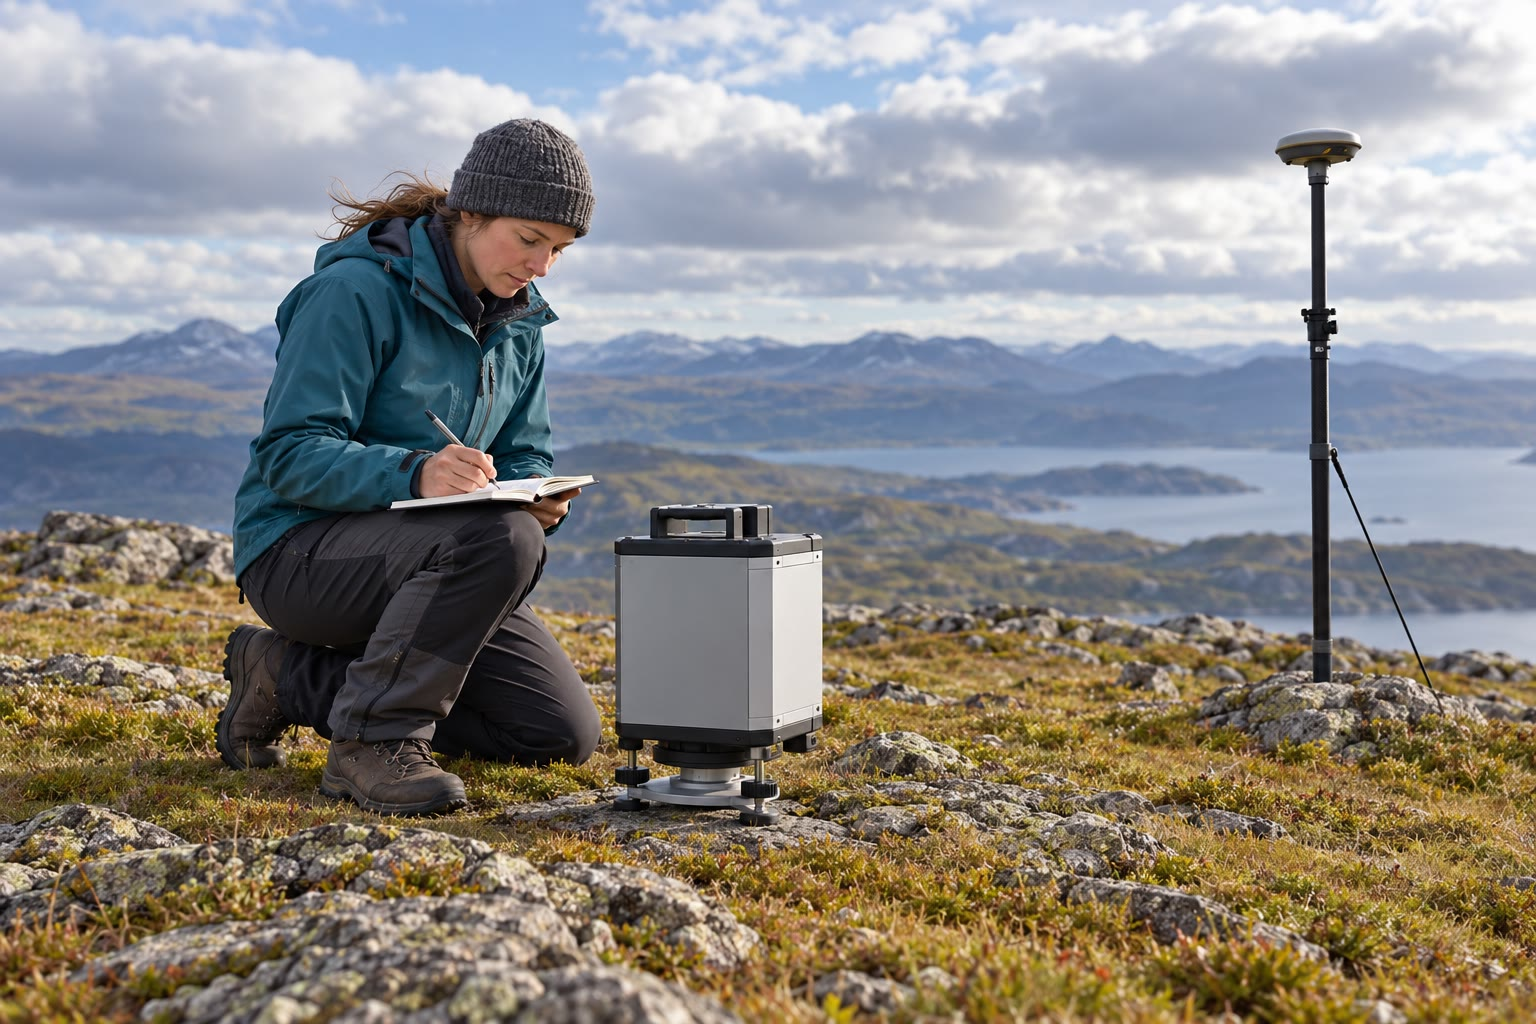
\includegraphics[width=\linewidth]{images/book5/ai/b3-gravimeter.jpg}

{\scriptsize مقياس جاذبية ميداني على قاعدة التسوية الخاصة به، مع
هوائي قمر صناعي في الخلفية (رسم توضيحي مولَّد بالذكاء الاصطناعي).}
\end{minipage}
\end{inthefield}

\section{التمارين}

\begin{exercise}[$\star$]\label{exo:b3:gravity-geodesy:1}
انطلاقًا من قيم نظام المرجع الجيوديسي 1980 $a = \qty{6378137}{m}$
و$f = \num{0.00335281068}$، احسب نصف المحور الأصغر $b$ و$a - b$. مع
$J_2 = \num{1.08263e-3}$ و$m = \num{0.00344979}$، احسب التفلطح الذي
تتنبّأ به علاقة كليرو، وقارِن.
\end{exercise}

\begin{exercise}[$\star$]\label{exo:b3:gravity-geodesy:2}
في سنةٍ جافة، يفقد حوض نهري مساحته \qty{5.0e5}{km^2} كتلةً قدرها \qty{60}{Gt} من
الماء. احسب التغيّر في \omterm{def:b3:gravity-geodesy:ewh}{ارتفاع الماء المكافئ}. بكم سيرفع الكتلة نفسها
مستوى سطح البحر، علمًا بأنّ \qty{360}{Gt} لكل مليمتر؟
\end{exercise}

\begin{exercise}[$\star$]\label{exo:b3:gravity-geodesy:3}
باستخدام المتسلسلة $\gamma = 9.780327(1 + 0.0053024\sin^2\varphi -
0.0000058\sin^22\varphi)$ \unit{m.s^{-2}}، احسب الجاذبية المرجعية عند
خطّ الاستواء، وعند \ang{45} وعند القطبين. عبّر عن الفرق بين القطب
والاستواء بالميليغال.
\end{exercise}

\begin{exercise}[$\star$]\label{exo:b3:gravity-geodesy:4}
احسب \omterm{def:b3:gravity-geodesy:flexure}{صلابة الانثناء} \omterm{def:b3:gravity-geodesy:alpha}{ومعامل الانثناء} للصفائح المحيطية حيث
$T_e = \qty{10}{km}$ و$T_e = \qty{30}{km}$ ($E = \qty{100}{GPa}$،
$\nu = 0.25$، $\rho_m - \rho_w = \qty{2270}{kg.m^{-3}}$، $g =
\qty{9.81}{m.s^{-2}}$). أين تقع حافة الحفرة المحيطة \omterm{def:b3:gravity-geodesy:alpha}{والانتفاخ الأمامي} تحت
حمل خطّي؟
\end{exercise}

\begin{exercise}[$\star\star$]\label{exo:b3:gravity-geodesy:5}
(أ) ارتفاع الجيود $+\qty{50}{m}$: احسب جهد الاضطراب هناك،
مستخدمًا $\gamma = \qty{9.80}{m.s^{-2}}$. (ب) على امتداد \qty{100}{km} يرتفع الجيود
بمقدار \qty{10}{m}. بأيّ زاوية يختلف خيط الشاقول هناك عن العمودي على
الإهليلجي؟ أعطِ الجواب بالثواني القوسية.
\end{exercise}

\begin{exercise}[$\star\star$]\label{exo:b3:gravity-geodesy:6}
انطلاقًا من $J_2 = \num{1.08263e-3}$ وعامل عزم القصور الذاتي
$C/(Ma^2) = \num{0.3308}$، احسب الانفراج الديناميكي $H = (C - A)/C$
و$1/H$. أيّ العددين يتغيّر لأرض متجانسة لها $J_2$ نفسه؟
\end{exercise}

\begin{exercise}[$\star\star$]\label{exo:b3:gravity-geodesy:7}
يدور قمر صناعي في مدار دائري على ارتفاع \qty{500}{km} فوق نصف القطر الاستوائي
($a = \qty{6378.137}{km}$، $GM = \qty{3.986005e14}{m^3.s^{-2}}$)، مائلًا بزاوية
\ang{89}. احسب دورَه ومعدّل تقدّم العقدة بالدرجات في اليوم.
لماذا تختار بعثات الجاذبية مدارات شبه قطبية؟
\end{exercise}

\begin{exercise}[$\star\star$]\label{exo:b3:gravity-geodesy:8}
لدينا شذوذان قيمة كلٍّ منهما \qty{10}{\milli\gal} عند السطح، وطولا موجتيهما
\qty{100}{km} و\qty{1000}{km}. احسب سعتيهما عند
ارتفاع \qty{500}{km}.
\end{exercise}

\begin{exercise}[$\star\star$]\label{exo:b3:gravity-geodesy:9}
نحو البحر من الخندق، تقع قمّة الانتفاخ الخارجي على بعد \qty{120}{km} من
محور الخندق. باعتماد نموذج الصفيحة المنكسرة مع وجود الماء فوقها، احسب
$\alpha$، $D$ و$T_e$، والمسافة التي تقطع عندها الصفيحة
مستواها غير المنثني.
\end{exercise}

\begin{exercise}[$\star\star\star$]\label{exo:b3:gravity-geodesy:10}
(أ) تحقّق من أنّ $w = w_0e^{-u}(\cos u + \sin u)$، حيث $u = x/\alpha$، يحقّق
$Dw'''' + (\rho_m - \rho_i)gw = 0$ من أجل $x > 0$، مع $\alpha$ كما هو معرَّف.
(ب) بيّن أنّ عزم الانحناء $-Dw''$ يبلغ أكبر قيمة له تحت الحمل ويغيّر
إشارته عند $x = \pi\alpha/4$. (ج) أين يُرجَّح أكثر أن تتشقّق الصفيحة عند
سطحها العلوي، ولماذا؟
\end{exercise}

\begin{exercise}[$\star\star\star$]\label{exo:b3:gravity-geodesy:11}
باعتماد $m = \num{0.00344979}$ و$C/(Ma^2) = \num{0.3308}$، اعكس
علاقة داروين--راديو لإيجاد التفلطح الهيدروستاتيكي. قارن مع
$f = \num{0.00335281}$: احسب الفرق والارتفاع الزائد لخطّ الاستواء
فوق الشكل الهيدروستاتيكي. ماذا يدلّ ذلك عن الوشاح؟
\end{exercise}

\begin{exercise}[$\star\star\star$]\label{exo:b3:gravity-geodesy:12}
يُراد لقمر صناعي على مدار دائري ارتفاعه \qty{700}{km} أن يحافظ على التوجّه نفسه
بالنسبة إلى الشمس طوال العام: يجب أن تتقدّم عقدته بمقدار \ang{360} في
سنة مدارية مدّتها \num{365.242}~يومًا. احسب ميل المدار المطلوب.
\end{exercise}

\section{مسألة: الحفرة المحيطة بظهرة أورو}

\begin{problem}[{مسألة نهاية الأسبوع --- شكل الأرض، وحمل بركاني،
حفرته الانثنائية وما تراه الأقمار الصناعية منها}]
\label{pb:b3:gravity-geodesy:1}
% values: calc/ch03.py; GRS80 (geod5:grs80-*), earth:MoI; flexure.py
أورو ظهرة بركانية متخيَّلة في محيط: سلسلة مستقيمة من براكين متلاحمة
طولها \qty{400}{km}، مبنية فوق الغلاف الصخري المحيطي القديم. ويُعتبر مقطعها
مثلثًا عرضه \qty{80}{km} عند قاعدته
وارتفاعه \qty{6}{km}، وكثافته \qty{2800}{kg.m^{-3}}، واقفًا على قاع بحر
عمقه \qty{5}{km}. كثافة الوشاح \qty{3300}{kg.m^{-3}}، وكثافة مياه البحر
\qty{1030}{kg.m^{-3}}، $E = \qty{100}{GPa}$، $\nu = 0.25$، $g =
\qty{9.81}{m.s^{-2}}$، $G = \qty{6.674e-11}{m^3.kg^{-1}.s^{-2}}$.

\medskip
\noindent\textbf{الجزء الأول --- شكل الأرض.} استخدم نظام
\babelsublr{Geodetic Reference System 1980}: $a = \qty{6378137}{m}$، $b = \qty{6356752.3}{m}$،
$GM = \qty{3.986005e14}{m^3.s^{-2}}$، $J_2 = \num{1.08263e-3}$،
$\omega = \qty{7.292115e-5}{rad.s^{-1}}$، $f = \num{0.00335281}$؛
و$C/(Ma^2) = \num{0.3308}$.
\begin{enumerate}
  \item احسب $m = \omega^2a^2b/(GM)$.
  \item احسب التفلطح الذي تعطيه علاقة كليرو انطلاقًا من $J_2$
        و$m$، ومقلوبه.
  \item احسب التفلطح الهيدروستاتيكي من علاقة داروين--راديو،
        ومقلوبه.
  \item قارن كليهما بالتفلطح المرصود. بكم مترًا يعلو
        خطّ الاستواء فوق الشكل الهيدروستاتيكي؟
  \item احسب الانفراج الديناميكي $H = (C - A)/C$.
\end{enumerate}

\noindent\textbf{الجزء الثاني --- الحمل.}
\begin{enumerate}[resume]
  \item احسب مساحة المقطع العرضي للظهرة.
  \item احسب الحمل الخطّي $V_0$، معتبرًا الظهرة كلّها مغمورة، بحيث
        يكون وزنها $(\rho_v - \rho_w)g$ لكلّ وحدة حجم.
  \item لو عُوّضت الظهرة محليًّا على طريقة إيري بجذرٍ من
        صخرها الخاص في الوشاح، فما عمق الجذر تحت
        القمّة؟
  \item لو كان التعويض موضعيًّا، لانتهى الجذر عند سفح الظهرة،
        على بعد \qty{40}{km} من محورها. تُظهر البيانات الباثيمترية حفرةً تمتدّ حتى
        \qty{165}{km}. ماذا يُستنتج من ذلك؟
\end{enumerate}

\noindent\textbf{الجزء الثالث --- الحفرة الانثنائية.} الحفرة مملوءة بالماء
($\rho_i = \rho_w$). يجد مقطع زلزالي عبر الظهرة أعلى
القشرة المحيطية عائدًا إلى عمقه الإقليمي على بعد \qty{165}{km} من المحور،
وقمّة \omterm{def:b3:gravity-geodesy:alpha}{الانتفاخ الأمامي} على بعد \qty{220}{km} من المحور.
\begin{enumerate}[resume]
  \item احسب \omterm{def:b3:gravity-geodesy:alpha}{معامل الانثناء} انطلاقًا من حافة الحفرة المحيطة.
  \item احسبه مرّة أخرى انطلاقًا من \omterm{def:b3:gravity-geodesy:alpha}{الانتفاخ الأمامي}. هل النتيجتان متّسقتان؟
  \item باعتماد $\alpha = \qty{70.0}{km}$، احسب \omterm{def:b3:gravity-geodesy:flexure}{صلابة الانثناء}.
  \item احسب \omterm{def:b3:gravity-geodesy:flexure}{السمك المرن الفعّال}.
  \item باعتماد $V_0 = \qty{4.17e12}{N.m^{-1}}$ و$D$ مقرَّبًا إلى ثلاثة
        أرقام معنوية، احسب الانخفاض تحت المحور.
  \item احسب ارتفاع \omterm{def:b3:gravity-geodesy:alpha}{الانتفاخ الأمامي}.
  \item تحقّق من أنّ الطفو لكامل الانخفاض، $2w_0\alpha(\rho_m -
        \rho_w)g$، يوازن $V_0$.
  \item قارن $T_e$ بالقيم المرصودة على طول ظهرة هاواي، من 17 إلى
        \qty{37}{km}. قارن الانخفاض تحت المحور مع
        جذر إيري في السؤال 8.
\end{enumerate}

\noindent\textbf{الجزء الرابع --- الجاذبية فوق الحفرة المحيطة.} خذ توافقيًّا واحدًا من
الانثناء، طول موجته $2\pi\alpha$ وسعته $W = \qty{500}{m}$، مُنحنيًا
كلًّا من قاع البحر (القشرة \qty{2900}{kg.m^{-3}} تحت الماء، على عمق \qty{5}{km} تحت
مستوى سطح البحر) والموهو (الوشاح تحت القشرة، على عمق \qty{12}{km} تحت مستوى سطح البحر). صفيحة
رقيقة ذات كثافة سطحية $\sigma$ تُنتج الشذوذ $2\pi G\sigma$
مباشرةً فوقها.
\begin{enumerate}[resume]
  \item احسب طول الموجة والعدد الموجي $k$ للتوافقي.
  \item احسب سعة الشذوذ عند مستوى سطح البحر الناتج عن قاع البحر المنحني
        بعد \omterm{prop:b3:gravity-geodesy:upward}{الاستمرار إلى الأعلى} من عمق \qty{5}{km}.
  \item احسب سعة الموهو المنحني، والمجموع الكلّي.
  \item احسب المجموع عند ارتفاع قمر صناعي، \qty{400}{km} فوق
        مستوى سطح البحر.
  \item بأيّ عامل يُضعَف توافقي طول موجته \qty{80}{km}، وهو عرض
        الظهرة، على ذلك الارتفاع؟ وماذا يمكن للقمر الصناعي أن يميّزه؟
  \item إلى أيّ درجة توافقية كروية $n \approx 2\pi R/\lambda$ يناظر
        التوافقي في السؤال 18 ($R = \qty{6371}{km}$)؟
  \item أعطِ \omterm{def:b3:gravity-geodesy:flexure}{السمك المرن الفعّال} للصفيحة تحت ظهرة
        أورو.
\end{enumerate}
\end{problem}
